\IEEEPARstart{H}{istopathology} plays a vital role in diagnostic medicine, as it involves the examination of tissue samples to identify and diagnose various diseases. The growing availability of digital histopathology images has led to increased efforts in developing machine learning-based techniques for automated image analysis. Among these techniques, Convolutional Neural Networks (CNNs) have demonstrated exceptional potential for accurate and efficient analysis of digital histopathology images (\cite{Wemmert2021DeepAnalysis}). However, like other machine learning approaches, CNNs may be prone to overfitting, causing them to become overly specialized to the training data and unable to generalize to new, unseen data. This is shown in the left part of figure \ref{doubledescent}. The phenomenon of "double descent" has emerged in recent years, describing a situation in which a model's performance initially improves, then worsens, and finally improves again as the model's capacity increases, this is shown in the right part of Figure \ref{doubledescent}.

\begin{figure}[!htb]
    \centering
    \begin{minipage}{0.45\textwidth}
        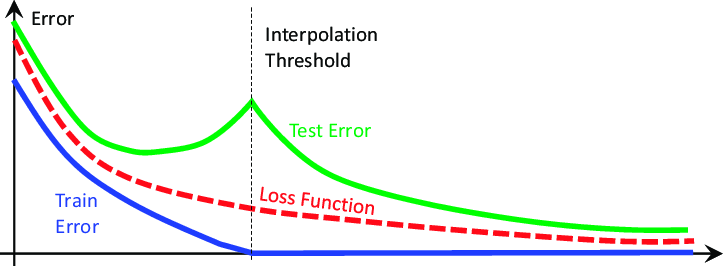
\includegraphics[width=\textwidth]{images/doubledescent.png}
        \caption{Example Double Descent in Test Error}
        \label{doubledescent}
    \end{minipage}
\end{figure}

This study aims to explore the relationship between a network's complexity and the presence of double descent in the context of histopathology image analysis. The central research question is: What is the relationship between the application of a more complex convolutional neural network and the presence of double descent for efficiency in identifying metastases in image patches from breast cancer patients? Understanding the potential advantages of double descent in CNN-based approaches is crucial for contributing to the development of more robust and effective automated image analysis tools for clinical practice, ultimately lowering the test error in diagnostic medicine. In this study, the complexity of the neural network is manipulated by varying the number of convolutional filters and dense layers used in the CNN architecture.


\subsection{Double Descent and Epoch-wise DoubleDescent}
Training a convolutional neural network (CNN) requires careful consideration due to the bias-variance trade-off, which is a fundamental concept in machine learning that describes the balance between a model's ability to fit the training data (bias) and its ability to generalize to new, unseen data (variance). Traditional machine learning conventions suggest that the ideal model complexity is achieved when the loss ceases to improve, falling within the classical U-shaped regime. However, recent studies on double descent propose that more accurate models can be obtained by surpassing the interpolation threshold, which occurs approximately when there are as many parameters as data points (\cite{Belkin2019ReconcilingTrade-off}). Beyond this threshold, models enter the "interpolation regime" or “Modern” over-parameterized regime, where an abundance of parameters allows for possible interpolation predictors, some of which are responsible for interpolation with low generalization error (\cite{Belkin2021FitInterpolation}).

A related phenomenon, termed epoch-wise double descent, can be observed during the training process in machine learning, specifically in the context of epoch-wise learning. Similar to double descent, epoch-wise double descent displays a characteristic descending and ascending pattern in model performance. However, this pattern only emerges when the model possesses sufficient complexity (\cite{Nakkiran2021DeepHurt, Stephenson2021WhenHappens}). The occurrence of epoch-wise double descent has significant implications for identifying the optimal stopping point during model training, as it may affect the model's ability to generalize to new, unseen data. This insight highlights the importance of carefully considering the training duration and model complexity to ensure the best possible performance in real-world applications.
%The appearance of a double descent has previously been shown by multiple studies: (\cite{Advani2017High-dimensionalNetworks, Neal2018ANetworks, Spigler2018AGeneralization})